\subsection{Contributions}
So far, the Riemannian Elevator and Kruskal's gradient descent algorithm have been implemented. The only thing that remains is adding the EKF to track points over time. Preliminary results show that even without the Kalman prediction step, the points are able to be tracked quite well. 

The EKF has yet to be implemented.
\subsection{Empirical Results}
Below are some graphs of empirical test using the implemented algorithms. Firstly, in figure~\ref{fig:kruskal} is a comparison between Kruskal's step size and $\frac{1}{\sqrt{k}}$ step. A number of robot positions and directions were generated, and their approximate positions were provided as initial guesses for the algorithms. After a set number of iterations or after the algorithms had converged, the robot moved a fixed distance in their chosen direction, and the algorithms we run again, this time with their previous guess as an initial guess.
\begin{figure}[ht]
    \centering
    \begin{subfigure}{\linewidth}
        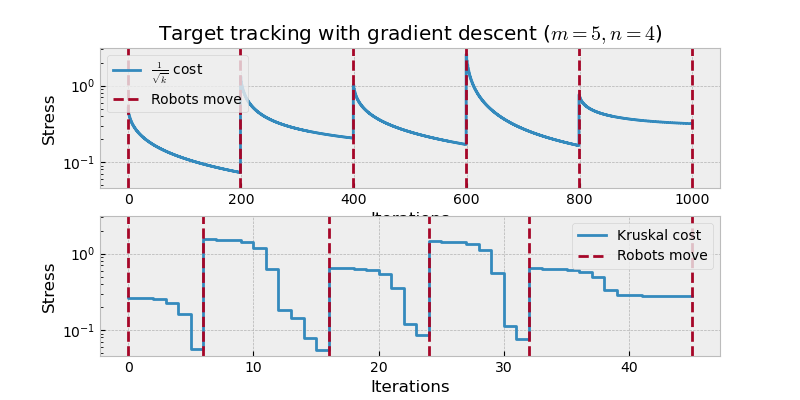
\includegraphics[width=\textwidth,trim=50 0 50 10, clip]{kruskal_5_4.png}
        \caption{Smaller tracking example with $n=4$ robots and $m=5$ measurements}
    \end{subfigure}
    \begin{subfigure}{\linewidth}
        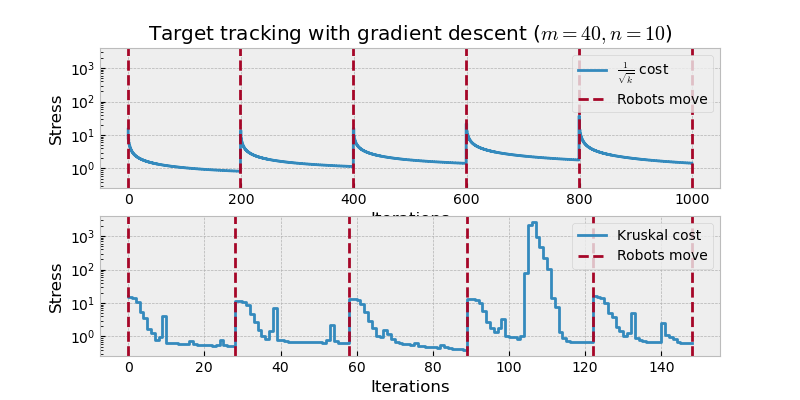
\includegraphics[width=\textwidth,trim=50 0 50 10, clip]{kruskal_40_10.png}
        \caption{Larger tracking example with $n=10$ robots and $m=40$ measurements}
    \end{subfigure}
    \caption{Two different cases of robot tracking. } \label{fig:kruskal}
\end{figure}

As is plainly visible in the graphs, Kruskal's algorithm vastly outperforms the standard step size in convergence rate. 

In figure~\ref{fig:riemann}, the point estimation from distance measurements is showcased. A number of points were generated with noisy distance measurements between them. These values were passed to the Riemannian elevator which generated an initial estimate of the positions, which were further refined by Kruskal's gradient descent method.

\begin{figure}[ht]
    \centering
    \begin{subfigure}{\linewidth}
        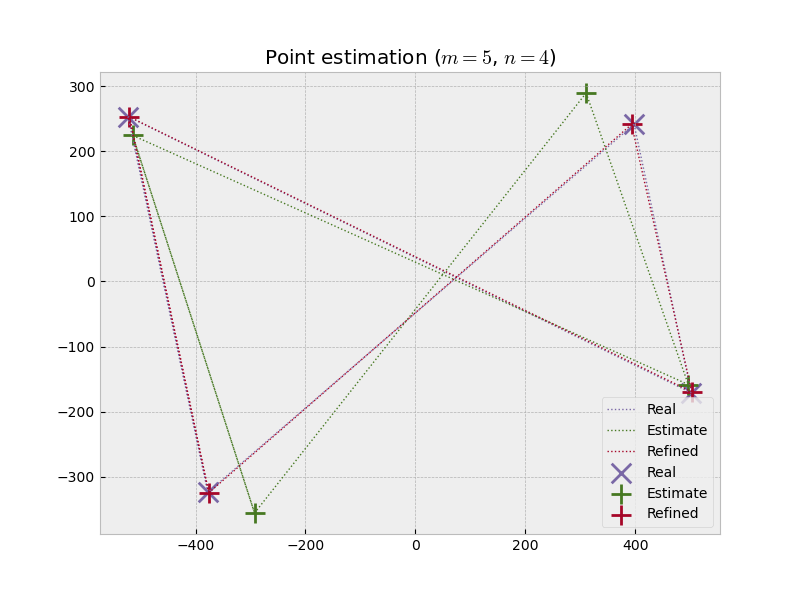
\includegraphics[width=\textwidth,trim=0 20 0 30, clip]{point_est_5_4.png}
        \caption{A smaller example of position estimation}
    \end{subfigure}
    \begin{subfigure}{\linewidth}
        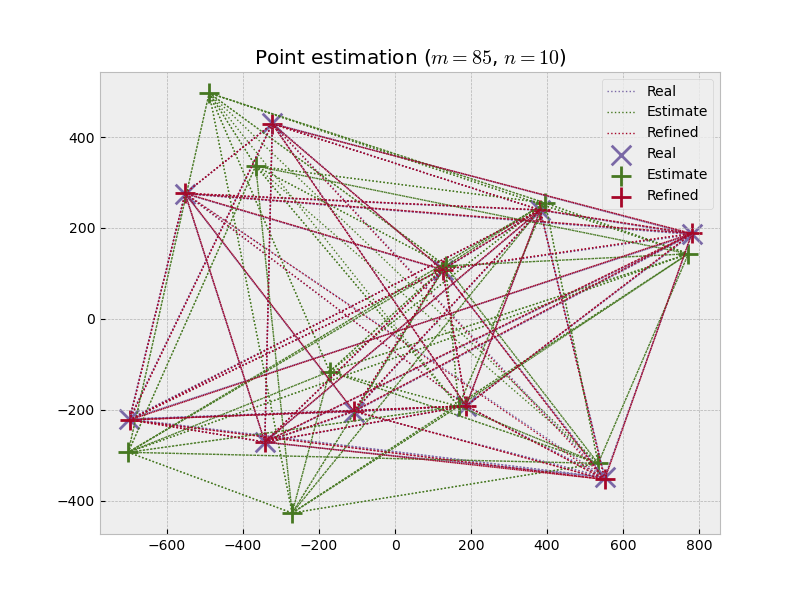
\includegraphics[width=\textwidth,trim=0 20 0 30, clip]{point_est_85_10.png}
        \caption{A larger example of position estimation}
    \end{subfigure}
    \caption{Position estimation from only distance measurements. While there is ambiguity in the rotation and positions of the estimates, they have been rotated and translated to align with the true value for clarity.} \label{fig:riemann}
\end{figure}

